\subsection{Graphical implementation}

One very important part in simulating a specific problem is visualization. First for checking if a given implementation makes sense the way one has written it, for bug fixing and for adjusting the parameters of the model to the real world problem.

\subsubsection{Preparatory work}
Before programming something out of the head one has to create an idea of how a problem could be implemented. One has to be careful to not exaggerate the model and fix too much on unimportant details, but to keep the main ideas clear and simple. 

\begin{figure}[htb]
	\centering
		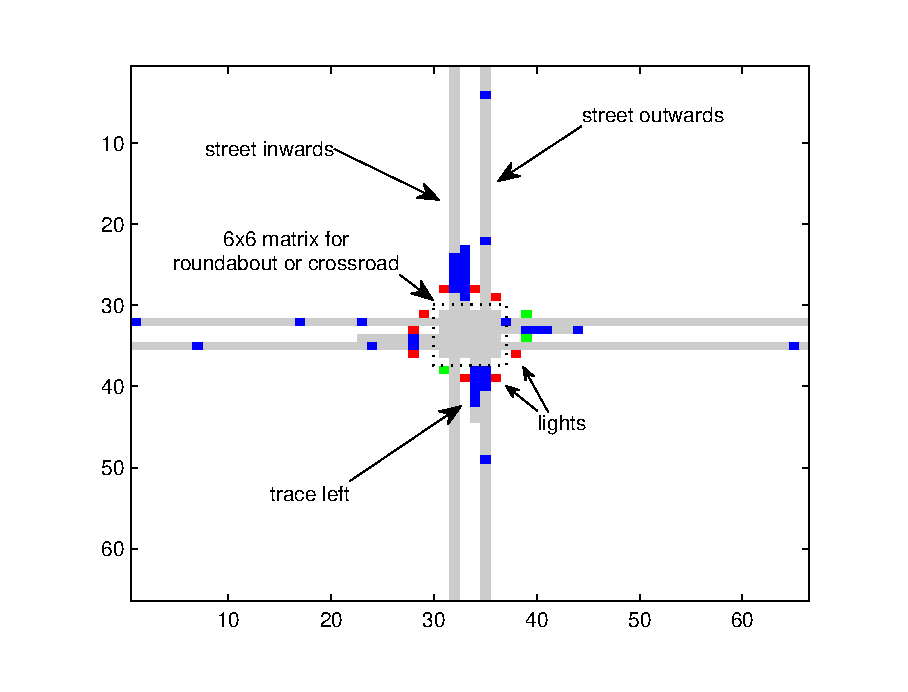
\includegraphics[width=0.8\textwidth]{images/description_mapping_overview.eps}
	\caption{Overview over the implementation of the plot.}
	\label{fig:description_mapping_overview}
\end{figure}

\autoref{fig:description_mapping_overview} shows how we finally ended in, because it shows the elementary cell of each intersection. Our model consisted of
\begin{itemize}
	\item a intersection (either roundabout or a crossroad)
	\item 8 streets for each direction of the crossroad (each with a out- and ingoing street)
	\item	pedestrians (not in the figure)
	\item	cars (in blue)
	\item	traffic lights for the cars and pedestrians in the case of a roundabout
	\item a trace for the cars that turn left in the case of a crossroad
\end{itemize}

In the following sections I will explain the programming details of this figure.

\subsubsection{Implementation}
For each type of intersections we have written a function that works out the paths of the cars and returns this information in a $6 \times 6$ matrix. Furthermore information about the pedestrians, the traffic light phases and the cars on the left trace are returned. I implemented these by creating a large matrix

\[
 \begin{split}
\mathrm{map} = (\mathrm{(No. \ of \ intersections \ in \ x \ direction)} \cdot (2 \cdot \mathrm{streetlength} + 6) \times \\ 
 \mathrm{(No. \ of \ intersections \ in \ y \ direction)} \cdot (2 \cdot \mathrm{streetlength} + 6))
\end{split}
\]

in which we wrote all elements listed up above for each time step, that we looked at. The elements of the maps were encoded in a color code from $0$ to $2$, i.e.
\begin{itemize}
	\item	Car = $0.6$
	\item	Red light = $1.6$
	\item	Pedestrian = $0.8$
\end{itemize}
that were written into this large matrix.
By plotting this matrix with
\begin{center}
\texttt{imagesc(map)}
\end{center}
and using a colormap we were able to create a relatively realistic model (see figure above).


\begin{figure}[htb]
	\centering
		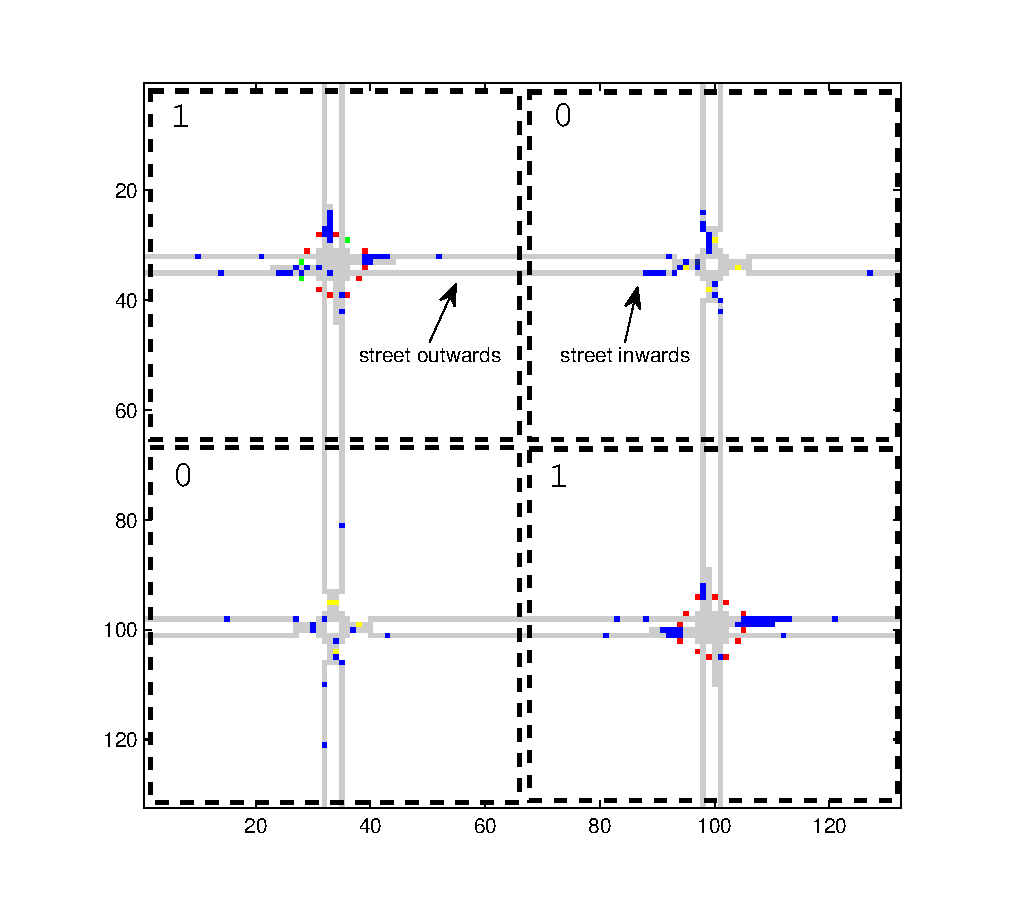
\includegraphics[width=0.8\textwidth]{images/description_mapping_detail.eps}
	\caption{Details about the implementation of the plot in the case of many intersections.}
	\label{fig:description_mapping_detail}
\end{figure}

We wanted to analyze how the traffic flow changes when we have many intersections in a map that are connected together to reproduce a more realistic view of the world. The configuration of each map was written into a matrix. This matrix had $0$ (corresponding to roundabout) and $1$ (corresponds to crossroad) as entries and corresponds to the rough structure of the map. Let's demonstrate this with \autoref{fig:description_mapping_detail}. We see in the top left and bottom right corners two crossroad and in the top right and bottom left corner two roundabouts. Naturally this would be denoted in a matrix as
\[
	\left(\begin{matrix}
1 & 0\\ 
0 & 1
\end{matrix}\right)
\]
and this is how we implemented it. Then the outgoing streets of the one cell are connected to the inwards streets of the neighboring cell and programing this, this results in these dynamic maps.

Furthermore we added the support of saving a video output of the this specific configuration. For further details see the code in the listings (see \autoref{plot_map}).

\newpage